% bilinear_interpolation.tex

\usetikzlibrary{calc}

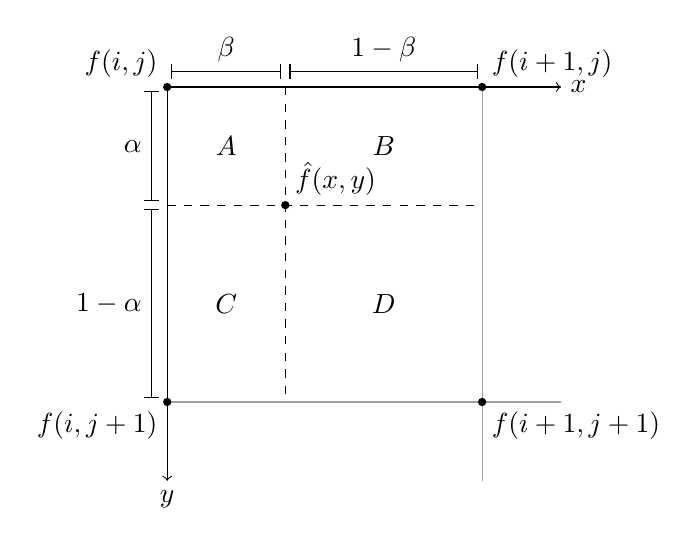
\begin{tikzpicture}
    \coordinate (O) at (0,0);
    \coordinate (P) at (1.5,-1.5);
    \coordinate (M) at (4,-4);

    \draw[gray!75] grid[step=4cm] (5, -5);

    \draw[->] (O) -- (5,0) node[right] {$x$};
    \draw[->] (O) -- (0,-5) node[below] {$y$};

    \fill (O) circle (1.5pt) node[above left] {$f(i,j)$};
    \fill (O-|M) circle (1.5pt) node[above right] {$f(i+1,j)$};
    \fill (M-|O) circle (1.5pt) node[below left] {$f(i,j+1)$};
    \fill (M) circle (1.5pt) node[below right] {$f(i+1,j+1)$};

    \fill (P) circle (1.5pt) node [above right] {$\hat{f}(x,y)$};

    \draw[dashed] (P|-O) -- (P|-M);
    \draw[dashed] (P-|O) -- (P-|M);

    \pgfmathsetmacro{\shift}{0.2}
    \draw[{[sep=1.5pt]|}-{[sep=1.5pt]|}] ([yshift=\shift cm]O) -- node[above]{$\beta$} ([yshift=\shift cm]O-|P);
    \draw[{[sep=1.5pt]|}-{[sep=1.5pt]|}] ([yshift=\shift cm]O-|P) -- node[above]{$1-\beta$} ([yshift=\shift cm]O-|M);

    \draw[{[sep=1.5pt]|}-{[sep=1.5pt]|}] ([xshift=-\shift cm]O) -- node[left]{$\alpha$} ([xshift=-\shift cm]O|-P);
    \draw[{[sep=1.5pt]|}-{[sep=1.5pt]|}] ([xshift=-\shift cm]O|-P) -- node[left]{$1-\alpha$} ([xshift=-\shift cm]O|-M);

    \node (A) at ($(O)!0.5!(P)$){$A$};
    \node (B) at ($(O-|P)!0.5!(P-|M)$){$B$};
    \node (C) at ($(O|-P)!0.5!(P|-M)$){$C$};
    \node (D) at ($(P)!0.5!(M)$){$D$};
\end{tikzpicture}